% Drawing 138/07-1 -- folder 138, batch 07, archive page 122 (PDF page 123).
% Transcription: une sphère ; sur l'équateur, en pointillé, le point $\infty$ ; en trait gras le segment de $0$ à $1$.
% Kind: dessin d'enfant on the sphere (segment 0 - 1). Method 3 (encoded, rendered from the data). Status: ok.
% Notes: A sphere; on the equator, its back half dotted, the point infinity; the segment from 0 to 1 in thick stroke along the front of the equator (a thinner arc above it closes a lens, drawn). Encoded as the trivial dessin: one edge from 0 (black) to 1 (white), one face (infinity), genus 0.
% Coordinates: 1 unit = 1 mm = 1/100 of the crop width (bbox in page fractions: [0.13, 0.36, 0.3, 0.46]).
% Redrawn by Claude (claude-opus-5-5), issue #73, 2026-11-07; not checked by a human; not compiled (no TeX in the session).
% Rights: reproduces part of the work -- behind RENDER_TRANSCRIPTS, never published by itself.
\documentclass[tikz,border=3pt]{standalone}
\usepackage{amsmath,amssymb}
\usetikzlibrary{patterns,arrows.meta}
\tikzset{pencil/.style={black!45}, struck/.style={black!35}, mark/.style={circle,draw,inner sep=1.3pt}, pt/.style={circle,fill,inner sep=0.9pt}, opt/.style={circle,draw,fill=white,inner sep=1.1pt}}
\begin{document}
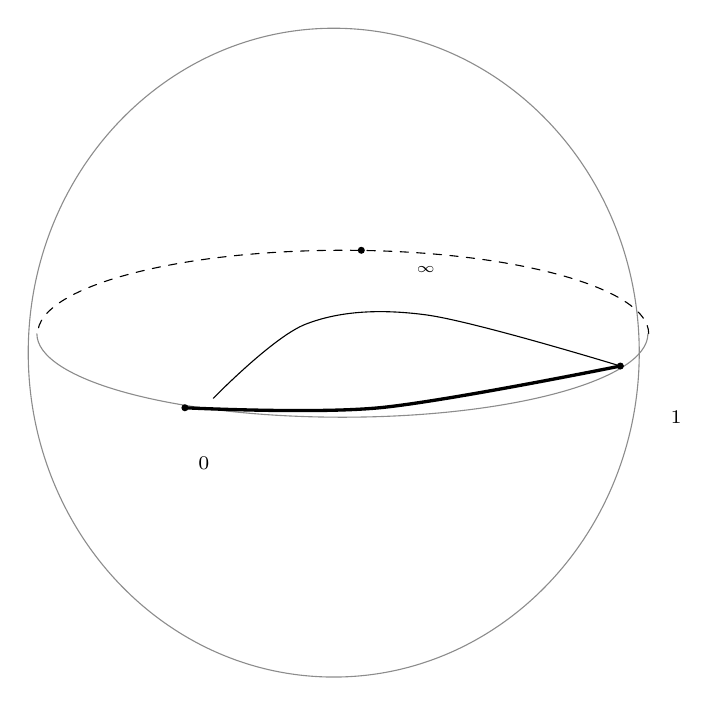
\begin{tikzpicture}[x=1mm,y=1mm,line cap=round,line join=round,font=\scriptsize]
\draw[pencil] (47.1,-42.4) ellipse[x radius=38.8, y radius=41.2];
\draw[dashed] (87.1,-40) arc[start angle=0, end angle=180, x radius=38.8, y radius=10.6];
\draw[pencil] (9.4,-40) arc[start angle=180, end angle=360, x radius=38.8, y radius=10.6];
\draw[very thick] plot[smooth, tension=0.55] coordinates {(28.2,-49.4) (52.9,-49.4) (83.5,-44.1)};
\draw plot[smooth, tension=0.55] coordinates {(31.8,-48.2) (43.5,-38.8) (58.8,-37.6) (83.5,-44.1)};
\node[pt] at (28.2,-49.4) {};
\node[pt] at (83.5,-44.1) {};
\node[pt] at (50.6,-29.4) {};
\node[inner sep=1pt] at (30.6,-56.5) {\scriptsize $0$};
\node[inner sep=1pt] at (90.6,-50.6) {\scriptsize $1$};
\node[inner sep=1pt] at (58.8,-31.8) {\tiny $\infty$};
\end{tikzpicture}
\end{document}
